\appendix{Sample Appendix}

\section{Width Based on Page Size Figure Example} \label{sec:appendxia_figure_example}
Here's an example of a figure whose width depends on the width
of the page. You can see if as Figure \ref{fig:appendix_some_pic}.

\begin{figure}[htbp]
  \centering
  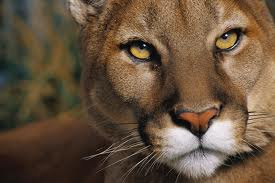
\includegraphics[width=0.45\textwidth,natwidth=610,natheight=642]{figures/appendixa/some_pic.jpg}
  \caption[Example Width Based on Page Size Figure]{
    This is an example of a figure whose width will be 45\% of the
    width of the page. If you'd like to see a figure with a fixed
    width then you can see it as Figure \ref{fig:intro_stuff} in
    Section \ref{sec:intro_figure_example}. Just FYI, I made this
    figure with PowerPoint and then copied it and pasted it into
    wmf2eps and choose the "Paste EMF" option. It will generate
    a larger file, but it will look a TON better than the
    "Paste WMF" option and the "Paste DIB" option will paste the
    rasterized image that won't scale well at all.}
  \label{fig:appendix_some_pic}
\end{figure}
